%%
%% Class homework & solution template for latex
%% Alex Ihler
%%
\documentclass[twoside,11pt]{article}
\usepackage{amsmath,amsfonts,amssymb,amsthm}
\usepackage{graphicx,color}
\usepackage{verbatim,url}
\usepackage{listings}
\usepackage{upquote}
\usepackage[T1]{fontenc}
%\usepackage{lmodern}
\usepackage[scaled]{beramono}
%\usepackage{textcomp}

% Directories for other source files and images
\newcommand{\bibtexdir}{../bib}
\newcommand{\figdir}{fig}

\newcommand{\E}{\mathrm{E}}
\newcommand{\Var}{\mathrm{Var}}
\newcommand{\N}{\mathcal{N}}
\newcommand{\matlab}{{\sc Matlab}\ }

\setlength{\textheight}{9in} \setlength{\textwidth}{6.5in}
\setlength{\oddsidemargin}{-.25in}  % Centers text.
\setlength{\evensidemargin}{-.25in} %
\setlength{\topmargin}{0in} %
\setlength{\headheight}{0in} %
\setlength{\headsep}{0in} %

\renewcommand{\labelenumi}{(\alph{enumi})}
\renewcommand{\labelenumii}{(\arabic{enumii})}

\theoremstyle{definition}
\newtheorem{MatEx}{M{\scriptsize{ATLAB}} Usage Example}

\definecolor{comments}{rgb}{0,.5,0}
\definecolor{backgnd}{rgb}{.95,.95,.95}
\definecolor{string}{rgb}{.2,.2,.2}
\lstset{language=Matlab}
\lstset{basicstyle=\small\ttfamily,
        mathescape=true,
        emptylines=1, showlines=true,
        backgroundcolor=\color{backgnd},
        commentstyle=\color{comments}\ttfamily, %\rmfamily,
        stringstyle=\color{string}\ttfamily,
        keywordstyle=\ttfamily, %\normalfont,
        showstringspaces=false}
\newcommand{\matp}{\mathbf{\gg}}




\begin{document}

\centerline{\Large Homework 2}
\centerline{Zachary DeStefano, 15247592}
\centerline{CS 274B: Spring 2016}

\section*{Problem 1: }

\subsection*{Part A,B}

Here is the code I used to produce the mutual information
\begin{lstlisting}
#Part A
D = np.genfromtxt('data/data.txt',delimiter=None)
loc = np.genfromtxt('data/locations.txt',delimiter=None)
m,n = D.shape # m = 2760 data points, n=30 dimensional

#Part B

#Find phat for each variable
posXcount = np.sum(D,axis=0)
probXj = np.zeros((n,2))
probXj[:, 1] = np.divide(posXcount,m)
probXj[:, 0] = 1-probXj[:,1]

#Find phat(x_j,x_k) for each pair of variables
probXjk = np.zeros((n,n,2,2))
for i in range(n):
    for j in range(n):
        for k in range(m):
            probXjk[i, j, D[k, i], D[k, j]] += 1
probXjk = np.divide(probXjk,m)

#Compute mutual information
mutualInfo = np.zeros((n,n))
for i in range(n):
    for j in range(n):
        curTerm = 0
        for k1 in range(2):
            for k2 in range(2):
                denomTerm = probXj[i,k1]*probXj[j,k2]
                jointTerm = probXjk[i, j, k1, k2]
                if denomTerm>0 and jointTerm>0:
                    curTerm += jointTerm*np.log(jointTerm/denomTerm)
        mutualInfo[i, j] = curTerm

#print results
print mutualInfo[0:5,0:5]
\end{lstlisting}

Here are the first 5 rows and columns of mutual information
\begin{lstlisting}
[[ 0.60870002  0.24584358  0.30645904  0.17521613  0.24642811]
 [ 0.24584358  0.66081843  0.28479996  0.21222061  0.29414659]
 [ 0.30645904  0.28479996  0.64609051  0.21486084  0.27873285]
 [ 0.17521613  0.21222061  0.21486084  0.68239551  0.23489376]
 [ 0.24642811  0.29414659  0.27873285  0.23489376  0.67286449]]
\end{lstlisting}

%\begin{figure}[h]
%\centering
%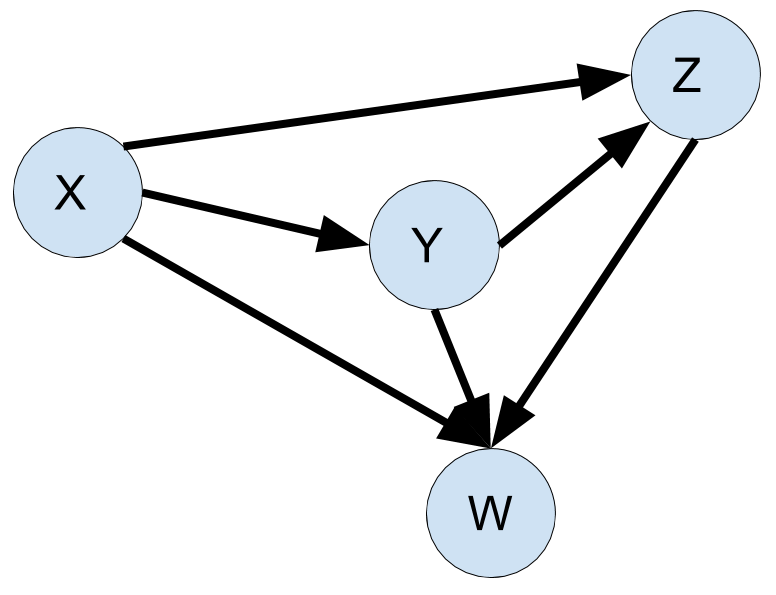
\includegraphics[width=3in]{HW1_Prob1_partA.png}
%\caption{Minimal Directed Graphical Model for Part A}
%\end{figure}
\section*{Problem 2:}

\subsection*{Part A}

\begin{lstlisting}
\end{lstlisting}


\end{document}
